\section{Experiments}

\begin{frame}{Experiments}
    \begin{itemize}
        \item Different parameter settings for each hypothesis
        \item Each experiment is run 100 times
        \item Experiment end statistics are written to files
        \item Test method: two-sample t-test % to determine whether the difference between means found in the sample is significantly different from the hypothesized difference between two means
        \item Significance level: 0.05
        \item Labels in plots show the independent variables that were varied
    \end{itemize}
\end{frame}


\begin{frame}{Experiments: Question 1 (1)}
    \begin{itemize}
        \item What is the relation between the amount of requests that RoboPizza receives and the waiting time for customers?
        \item[]
        \item $\mu_1$: mean waiting time for lower amount of requests
        \item $\mu_2$: mean waiting time for higher amount of requests
        \item[]
        \item $H_0$: The waiting time does not increase with the amount of requests ($\mu_1 \geq \mu_2$)
        \item $H_1$: The waiting time increases with the amount of requests ($\mu_1 < \mu_2$)
    \end{itemize}
\end{frame}

\begin{frame}{Experiments: Question 1 (2)}
    \begin{columns}

        \begin{column}{0.5\textwidth}
            \begin{itemize}
                \item Total task waiting time
            \end{itemize}

            \begin{figure}[hbt]
                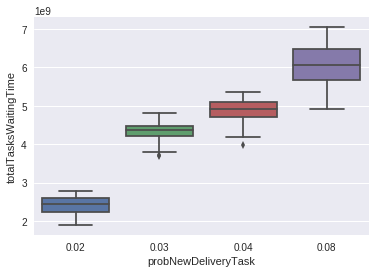
\includegraphics[width=1.1\textwidth]{img/question1-plot1}
            \end{figure}
        \end{column}

        \begin{column}{0.5\textwidth}
            \begin{itemize}
                \item $\mu_1 \geq \mu_2$
                    \begin{itemize}
                        \item t-value = 56.908
                        \item p-value = 0.000
                        \item $\rightarrow$ Reject $H_0$
                    \end{itemize}

                \item $\mu_2 \geq \mu_3$
                    \begin{itemize}
                        \item t-value = 14.425
                        \item p-value = 0.000
                        \item $\rightarrow$ Reject $H_0$
                    \end{itemize}

                \item $\mu_3 \geq \mu_4$
                    \begin{itemize}
                        \item t-value = 21.355
                        \item p-value = 0.000
                        \item $\rightarrow$ Reject $H_0$
                    \end{itemize}
            \end{itemize}
        \end{column}

    \end{columns}
\end{frame}



\begin{frame}{Experiments: Question 2 (1)}
    \begin{itemize}
        \item Do robots drive more (non-idle time) when there are more requests in the system?
        \item[]
        \item $\mu_1$: mean travel time for lower amount of requests
        \item $\mu_2$: mean travel time for higher amount of requests
        \item[]
        \item $H_0$: Robots do not drive more when there are more requests in the system ($\mu_1 \geq \mu_2$)
        \item $H_1$: Robots drive more when there are more requests in the system        ($\mu_1 < \mu_2$)
        \item[]
        \item Interesting to check if communication overhead for task distribution increases under high load
    \end{itemize}
\end{frame}

\begin{frame}{Experiments: Question 2 (2)}
    \begin{itemize}
        \item Total tasks and robot idle time
    \end{itemize}

    \begin{figure}[!hbt]
        \begin{adjustbox}{center}
            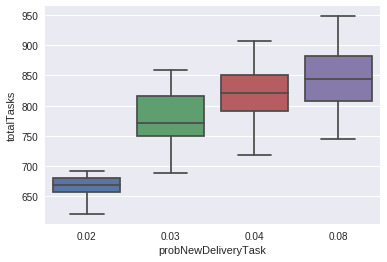
\includegraphics[width=6cm]{img/question2-plot3}
            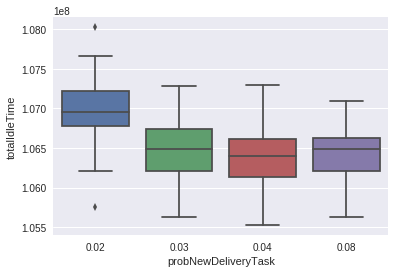
\includegraphics[width=6cm]{img/question2-plot1}
        \end{adjustbox}
    \end{figure}
\end{frame}

\begin{frame}{Experiments: Question 2 (3)}
    \begin{columns}

        \begin{column}{0.5\textwidth}
            \begin{itemize}
                \item Total travel time
            \end{itemize}

            \begin{figure}[hbt]
                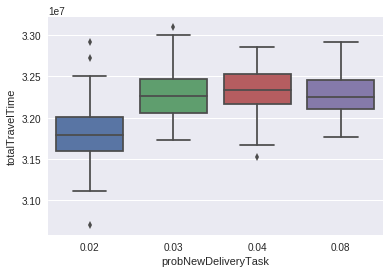
\includegraphics[width=1.1\textwidth]{img/question2-plot2}
            \end{figure}
        \end{column}

        \begin{column}{0.5\textwidth}
            \begin{itemize}
                \item $\mu_1 \geq \mu_2$
                    \begin{itemize}
                        \item t-value = 10.583
                        \item p-value = 0.000
                        \item $\rightarrow$ Reject $H_0$
                    \end{itemize}

                \item $\mu_2 \geq \mu_3$
                    \begin{itemize}
                        \item t-value = 0.590
                        \item p-value = 0.556
                        \item $\rightarrow$ Cannot reject $H_0$
                    \end{itemize}

                \item $\mu_3 \geq \mu_4$
                    \begin{itemize}
                        \item t-value = -0.582
                        \item p-value = 0.561
                        \item $\rightarrow$ Cannot reject $H_0$
                    \end{itemize}
            \end{itemize}
        \end{column}

    \end{columns}
\end{frame}



\begin{frame}{Experiments: Question 3 (1)}
    \begin{itemize}
        \item Does increasing the amount of robots decrease customer waiting time when there are many requests ($p_{task} = 0.04$)?
        \item[]
        \item $\mu_1$: mean waiting time for lower amount of robots
        \item $\mu_2$: mean waiting time for higher amount of robots
        \item[]
        \item $H_0$: Increasing the amount of robots does not decrease customer waiting time when there are many requests ($\mu_1 \geq \mu_2$)
        \item $H_1$: Increasing the amount of robots decreases customer waiting time when there are many requests ($\mu_1 < \mu_2$)
        \item[]
        \item Interesting to see the effect of more robots under high load. Higher load and more robots each cause more communication.
    \end{itemize}
\end{frame}

\begin{frame}{Experiments: Question 3 (2)}
    \begin{columns}

        \begin{column}{0.5\textwidth}
            \begin{itemize}
                \item Total task waiting time
            \end{itemize}

            \begin{figure}[hbt]
                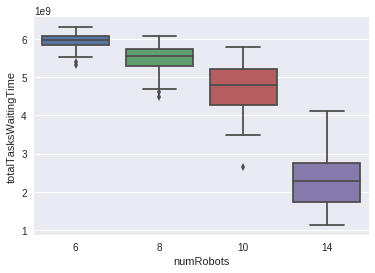
\includegraphics[width=1.1\textwidth]{img/question3-plot1}
            \end{figure}
        \end{column}

        \begin{column}{0.5\textwidth}
            \begin{itemize}
                \item $\mu_1 \geq \mu_2$
                    \begin{itemize}
                        \item t-value = -12.150
                        \item p-value = 0.000
                        \item $\rightarrow$ Cannot reject $H_0$
                    \end{itemize}

                \item $\mu_2 \geq \mu_3$
                    \begin{itemize}
                        \item t-value = -11.090
                        \item p-value = 0.000
                        \item $\rightarrow$ Cannot reject $H_0$
                    \end{itemize}

                \item $\mu_3 \geq \mu_4$
                    \begin{itemize}
                        \item t-value = -24.925
                        \item p-value = 0.000
                        \item $\rightarrow$ Cannot reject $H_0$
                    \end{itemize}
            \end{itemize}
        \end{column}

    \end{columns}
\end{frame}



\begin{frame}{Experiments: Question 4 (1)}
    \begin{itemize}
        \item How do waiting times change as the amount of road works changes (dynamism)?
        \item[]
        \item $\mu_1$: mean waiting time for lower amount of road works
        \item $\mu_2$: mean waiting time for higher amount of road works
        \item[]
        \item $H_0$: Waiting times do not increase as the amount of road works increases ($\mu_1 \geq \mu_2$)
        \item $H_1$: Waiting times increase as the amount of road works increases ($\mu_1 < \mu_2$)
        \item[]
        \item Interesting to see how the system copes with dynamism
    \end{itemize}
\end{frame}

\begin{frame}{Experiments: Question 4 (2)}
    \begin{itemize}
        \item Total road works and delivery tasks
    \end{itemize}

    \begin{figure}[!hbt]
        \begin{adjustbox}{center}
            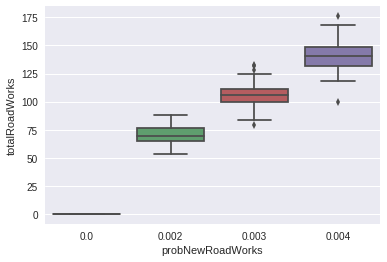
\includegraphics[width=6cm]{img/question4-plot1}
            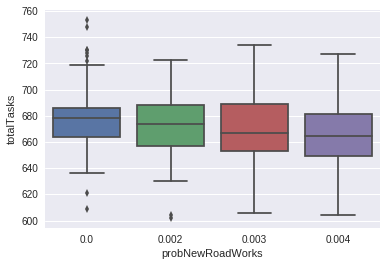
\includegraphics[width=6cm]{img/question4-plot2}
        \end{adjustbox}
    \end{figure}
\end{frame}

\begin{frame}{Experiments: Question 4 (3)}
    \begin{columns}

        \begin{column}{0.5\textwidth}
            \begin{itemize}
                \item Total task waiting time
            \end{itemize}

            \begin{figure}[hbt]
                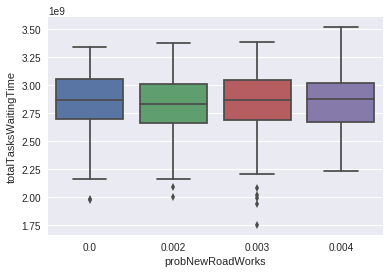
\includegraphics[width=6cm]{img/question4-plot3}
            \end{figure}
        \end{column}

        \begin{column}{0.5\textwidth}
            \begin{itemize}
                \item $\mu_1 \geq \mu_2$
                    \begin{itemize}
                        \item t-value = -0.636
                        \item p-value = 0.525
                        \item $\rightarrow$ Cannot reject $H_0$
                    \end{itemize}

                \item $\mu_2 \geq \mu_3$
                    \begin{itemize}
                        \item t-value = 0.391
                        \item p-value = 0.696
                        \item $\rightarrow$ Cannot reject $H_0$
                    \end{itemize}

                \item $\mu_3 \geq \mu_4$
                    \begin{itemize}
                        \item t-value = 0.732
                        \item p-value = 0.465
                        \item $\rightarrow$ Cannot reject $H_0$
                    \end{itemize}
            \end{itemize}
        \end{column}

    \end{columns}
\end{frame}

